\chapter{Experiments}
\label{cha:Experiments}

\section{Evaluation metrics}

\subsection{success\_rate}
The primary metric of evaluation for the developed agents is the $success\_rate$. The $success\_rate$ is defined as the ratio of successful episodes to the total number of episodes. An episode is considered successful if the agent passes through all three goals within the time limit \ref{time_limit}. Collisions of the agent do not disqualify an episode from being succesful, as long as the agent passes all goals.

\subsection{goal\_completion\_rate}

The $goal\_completion\_rate$ is defined as the ratio of passed goals to the total number of goals in the episodes. The $goal\_completion\_rate$ is a more fine-grained metric than the $success\_rate$. However the two metrics are closely related as a high $success\_rate$ implies a high goal\_completion\_rate. The major advantage of the $goal\_completion\_rate$ is that it can used to measure the progress of an agent during training more accurately. 
The $goal\_completion\_rate$ would increase when the agent is able to pass more goals on average, whereas the $success\_rate$ would only increase when the agent is able to pass all goals in an episode more often. The $goal\_completion\_rate$ captures learning progress earlier in training. This behaviour can be observed in training runs, shown in \ref{fig:success_rate_vs_goal_completion_rate}.


\begin{figure}
    \centering
    \subfigure[success\_rate]{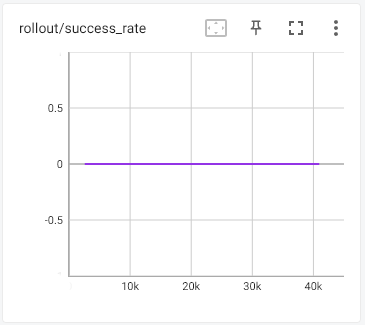
\includegraphics[width=0.3\textwidth]{Bilder/metrics/sr_vs_gcr_success_rate.PNG}}
    \subfigure[goal\_completion\_rate]{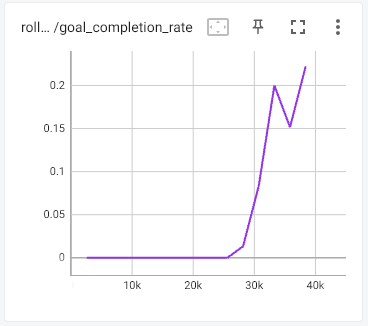
\includegraphics[width=0.3\textwidth]{Bilder/metrics/sr_vs_gcr_goal_completion_rate.PNG}}
    \caption{Difference in success rate and goal completion rate during early stages of training.}
    \label{fig:success_rate_vs_goal_completion_rate}
\end{figure}
% diese Bilder funktionieren nur für frühe Episoden, später sind die Werte sehr gleich

\subsection{collision\_rate}

The $collision\_rate$ is defined as the ratio of episodes with one or more collisions to the total number of episodes. The $collision\_rate$ is a measure of the agent's ability to avoid obstacles. The $collision\_rate$ is a secondary metric. The $collision\_rate$ is used in combination with the $success\_rate$ to determine the agent's performance.
The collision rate is also very useful during the training of the agent. If the agent's goal completion rate is low and there are no collisions, the agent might be stuck in a local optimum. In one such situation, the agent turned on the spot avoiding any collisions and did not move forward at all.
The collision rate can be used to detect such situations, the training process can then be adjusted accordingly.


\section{Basic evaluation algorithm}
\label{sec:eval_model_track}

This section explains most important component of the evaluation algorithms. It explains how the policy's performance is evaluated on a specific light and difficulty setting. The sampling mode and jetbot name can also be specified. This basic component is widely used in the following tests.

The agent is evaluated by running a fixed number of episodes for the specific light and difficulty settings. The amount of episodes that the agent is evaluated on is defined by the config parameter $n\_eval\_episodes$. As described in \ref{cha:env_description}, each difficulty setting includes a number of unique tracks. Furthermore the initial starting rotation is parameterized by the config parameter $spawn\_point$.

The tracks and starting positions for the agent are generated by the algorithm shown in \ref{fig:generate_track_rotation}. The algorithm divides the random interval specified by the spawn point parameter into $n\_eval\_episodes$ equal parts. These spawn rotations are then each assigned a track in repeating order.
This algorithm ensures that the agent is evaluated on the full range of unique tracks and spawn points.
It also makes the evaluations comparable, as the same combinations of tracks and spawn points are used for each agent evaluation.

The evaluation algorithm initializes $n\_eval\_episodes$ environments with the specified light settings. The obstacles and agents are then placed in the environments according to the generated map and rotation pairs. The evaluation episodes are started and the agents act in their environment until their episodes are terminated. The agent's actions are sampled deterministically or non-deterministically depending on the function call's parameter.
The $success\_rate$ and other metrics are calculated from the executed episodes.

% TODO deterministic parameter

\section{Question 1 - Model evaluation track difficulties}

The agent is evaluated on all three different difficulty settings to determine if the agent is successful in completing the tracks.
The Basic evaluation algorithm is used with the standard light setting for each of the three difficulty settings.
The policy is executed in non deterministic mode. This mode showed slight improvements over deterministic sampling, see \ref{sec:deterministic_check}



\paragraph{Test parameters}

100 episodes are evaluated for every difficulty setting. The $spawnOrientation$ from the training process is reused for the evaluation. 


\section{Question 2 - Model evaluation all light settings}

The agent is evaluated on every combination of light and difficulty settings. The Basic evaluation algorithm is used for these evaluations.
The $success\_rate$ metric is collected for each combination of light and difficulty settings separately. The collected $success\_rates$ are then averaged to produce aggregate $success\_rates$ for each light setting and difficulty setting as well as the $total\_success\_rate$. All collected and aggregate $success\_rates$ are shown in \ref{table:success_rates_system}.
The experiment shwos if the agent is able to adapt to different light settings and if the agent's performance is influenced by the light settings.

\begin{table}
\begin{center}
\resizebox{\textwidth}{!}{%
\begin{tabular}{|| c | c | c | c | c ||} 
    \hline
    \makecell{} & bright & standard  & hard & \makecell{aggregate \\ success\_rates} \\ [0.5ex] 
    \hline\hline
    \makecell{easy} &  success\_easy\_bright & success\_easy\_standard & success\_easy\_dark & success\_easy \\ 
    \hline
    \makecell{medium} &  success\_medium\_bright & success\_medium\_standard & success\_medium\_dark & success\_medium \\ 
    \hline
    \makecell{hard} &  success\_hard\_bright & success\_hard\_standard & success\_hard\_dark & success\_hard \\ 
    \hline
    \makecell{aggregate \\ success\_rates}  & success\_bright & success\_standard & success\_dark & total\_success\_rate \\
    \hline
\end{tabular}}
\end{center}
\caption{Collected and aggregate success\_rate metrics}
\label{table:success_rates_system}
\end{table}


\section{Question 3 - Investigating the feasibility of transfering the policy to a physical robot.}

Previous sections describe how a policy was developed that can be used to control an agent in a simulated environment. This section describes how I will investigate the feasibility of transfering the developed policy onto physical devices. The simulated agent was modeled after a Nvidia JetBot. The Nvidia JetBot is a small robot that is equipped with a camera, a processing unit and two motors that can be controlled independently. 
The Nvidia Jetbot is designed to be able to execute AI software. However the limited computational power of the JetBot raises the question whether the developed policy can be transfered to the JetBot. 

The developed policy takes a camera image from the front of the agent as input and applies preprocessing steps to the image. The preprocessed image is then processed by a convolutional neural network that outputs two acceleration values, one for each motor. The acceleration values are applied to the motors for a fixed amount of time. While the agent is moving, the camera image is constantly updated and the policy is applied to the new image. It is crucial that the agent's policy can be computed quick enough to be able act in real time. 

\subsection*{Effects of insufficiently slow policy computation}
If the jetbot is not able to compute the developed policy in the required time, there are two options that do not require changes to the developed/trained policy. The first option is to stop the motors until the policy is computed and then apply the acceleration values. This would make the jetbot movement overall slower and less smooth.
The second option is to apply the last computed acceleration values to the motors until the new policy is computed. This could result in a degradation of the jetbot's performance since the actions would be less accurate.
The two options are shown with visual representations in \ref{fig:slow_policy_computation}.


% gif splitter
% https://ezgif.com/split


\newcommand{\spc}[2]{\subfigure[#1]{\includegraphics[width=0.2\textwidth]{Bilder/slow_policy_computation/#2.png}}}
%\newcommand{\spc}[2]{\begin{subfigure}{.5\textwidth}\centering\includegraphics[width=0.2\textwidth]{Bilder/slow_policy_computation/#2.png}\caption*{#1}\end{subfigure}}
% trying to remove a), b) ... https://tex.stackexchange.com/questions/165508/remove-a-b-from-subfigure-numbering-but-keep-the-subfigure-caption

\begin{figure}
    
    \begin{center}
    \begin{tabular}{|| c | c | c ||} 
        \hline
        Policy computation in time & \makecell{Option 1: \\ Wait} & \makecell{Option 2:\\ Apply previous outputs}  \\ [0.5ex] 
        \hline\hline
        \spc{Start}{start} &  \spc{Start}{start} & \spc{Start}{start} \\ 
        \hline
        \spc{Agent turns right}{agent_turns_right} & \spc{Agent turns right}{agent_turns_right} & \spc{Agent turns right}{agent_turns_right} \\
        \hline
        \spc{Agent stops turning and goes strait}{agent_turns_left} & \spc{Agent waits}{agent_turns_right} & \spc{Agent continues to turn}{agent_fails_to_turn_left} \\
        \hline
        \spc{Agent continues}{agent_continues_properly}  & \spc{Agent stops turning and goes strait}{agent_turns_left} & \spc{Agent crashes}{agent_crashes} \\
        \hline
        \makecell{Agent moves properly.}  & \makecell{Agent overall speed is reduced.} & \makecell{Agent behaviour is changed.} \\
        \hline
    \end{tabular}
    \end{center}
    \caption{Possible effects of slow policy computation on the performance.}
    \label{fig:slow_policy_computation}
\end{figure}



\subsection{Policy Replay Experiment}
\label{sec:experiments_policy_replay}

This experiment examines the processing capabilities of the Nvidia Jetbot in the context of policy computation. The goal of this experiment is to determine if the policy can be computed on the jetbot hardware in real time. This would allow for a transfer of the developed policy to the physical agent without resorting to the two options highlighted in the previous section.

The experiment is conducted by recording the agent's actions in simulation and replaying them on the Nvidia Jetbot. The experiment measures the time it takes to replay the recorded actions on the jetbot. 

\paragraph{Recording Episodes}

Episodes are recorded in the simulation environment. The policy that is used for the recording is saved for later replay on the jetbot.
The recordings consist of the agent's camera images and the corresponding policy outputs. The camera images are saved without the proprocessing steps applied. These images represent the raw camera input that the jetbot agent would recieve in real time. The policy outputs are saved to verify the accuracy of the policy on the jetbot.

The episode recordings and policy are then transfered to the jetbot and executed. 

\paragraph{Replaying Episodes}

The recorded episodes are replayed on the jetbot. The policy from the recording is used to execute the replays on the jetbot. All recorded images and policy outputs are loaded into memory in preparation of an episode replay. 
The episodes are replayed step by step. The replay of a step consists of all the processing to obtain new acceleration values from a camera image. Image preprocessing and memory mechanism are executed for each step according to the specifications of the saved policy. The policy outputs are then computed. The computed policy outputs and the recorded policy outputs are used to verify the accuracy of the saved policy on the jetbot. 

The transfer of a neural network to a new device can result in different outputs due to different hardware. The computed and saved policy outputs are compared to determine the accuracy of the policy on the jetbot.

The test measures the time it takes to replay the recorded steps on the jetbot.
The measured times are compared against the $fixedTimestepsLength$ parameter of the recorded policy.


\paragraph{Test Dataset}

Episodes of all difficulty and light setting combinations are recorded to have a diverse set of data to evaluate. The episodes are recorded with the same policy as question 1 and 2, the most successful policy.

% we always record in the use_fresh_obs mode


\section{Other Experiments}

\subsection{Sampling mode performance test}
\label{sec:deterministic_check}

The PPO policy produces an action distribution when given an input observation. The action distribution is sampled to obtain an action for the agent to execute in the environment. The distribution can be sampled deterministically or non-deterministically. Deterministic sampling returns the most likely action, indicated by the mean of the distribution. Non-deterministic sampling returns a sample from the distribution according to the distribution's probabilities. This results in different output actions for the same observations. The PPO policy uses non-deterministic sampling during training to explore the action space. 

While the exploration caused by non-deterministic sampling is beneficial during training, it could be detrimental during evaluation. This exploration could lead the agent to take actions that are not optimal for the given observation and result in a lower $success\_rate$. Non-deterministic sampling can also be used during evaluation to reduce overfitting. This has been used in the Atari paper \autocite{atari} and the human-level control paper \autocite{human_level_control}. The environments examined in these papers are deterministic with identical starting states. Therefore a deterministic policy would result in identical results for the individual evaluation episodes.

Due to the difference in environment properties between the JetBot environment and the Atari environment, it is not clear if deterministic or non-deterministic sampling is better for the JetBot environment. The sampling mode performance test evaluates the agent with deterministic and non-deterministic sampling to determine if the agent's performance is affected by the sampling method. 

The sampling mode performance test uses the Basic evaluation algorithm to evaluate an agent with derministic and non-deterministic sampling for each difficulty level. The test evaluates the agents only using the standard light setting to save evaluation time. The success rates for the two sampling modes are compared to determine if the agent's performance is influenced by the sampling method.



% atari.pdf and human_level_control.pdf uses epsilon greedy during evals (their environment is deterministic, thus using a deterministic policy would result in the same results for every episode)

% default we use non deterministic, as that has shown (slightly) better results and is also used by atari paper


\subsection{Identical start condition Test}

rewrite this test to do the basic evaluation algorithm multiple times and find this way if accurate?
the current implementation might suffer from the specific chosen episode start params (see python results folder) TODO
or reexecute the test to see if the results are consistent

% TODO the policy is also non-determinsitic during the eval runs, so the purpose of this test is a bit different (first paragraph)
The environment is simulated in Untiy and was described in \ref{cha:env_description} to not be fully deterministic. This means identical actions in identical environments could result in different outcomes. These changes are small, such as changes to a few pixels in the agent camera. However these small changes might result in different agent actions. These actions further influence the environment and following actions. This means that episodes with identical starting conditions could result in different outcomes. This could be problematic when evaluating the agent, as the agent's performance could be influenced by the environment's randomness. 

The identical start condition test evaluates the agent on multiple episodes with identical starting conditions. The episode results are analysed to see if the policy is consistent when given identical starting conditions. If the policy is inconsistent given identical starting conditions the evaluation results according to \ref{sec:eval_model_track} are not reliable. The evaluation algorithm described in \ref{sec:eval_model_track} evaluates the agent on a series of different starting conditions, each starting condition is unique and only evaluated once.

This test runs multiple episodes with identical start conditions and analyses the episodes. The episode results are characterized and grouped. The groups are then analysed to determine if the agent's performance is consistent given identical starting conditions. A low number of groups indicates that the agent's performance is consistent. Ideally there is only one group that all episode results belong to.
The episode results are characterized by the endEvent, collision and the three goals' completion.



\subsection{Fresh Observation Test}

In the standard reinforcement learning algorithms each step transition results in a new observation that represents the environment's new state. Calls to the Unity environment and the step transitions in the environment take time. In order to speed up the training process the step calls to the simulated environment have been implemented in a non-blocking way. This means the step calls return before the entire step transition has been completed. The observation after the step transition is not yet available when the call returns. The observation returned by the step call is the observation of the environment at the beginning of the step transition. This observation does not capture the changes that have occurred in the environment during the step transition. The full changes are then visible to the agent after the next step has completed. 

The option $use\_fresh\_obs$ controls what observations the policy uses to produce the next actions. If $use\_fresh\_obs$ is set to false, the observation returned by the last step call is used. If $use\_fresh\_obs$ is set to true, a new observation is requested from the Unity simulation.

The fresh observation test evaluates a trained policy with both $use\_fresh\_obs$ settings to determine if the agent's performance is influenced by the freshness of the observations. The trained policy used one setting of the $use\_fresh\_obs$ parameter during training. The test shows if there is a difference in the agent's performance when using the other setting. The test evaluates the agent on light and difficulty settings following the evaluation algorithm described in \ref{sec:eval_model_track}.


% ## fresh obs better than nonfresh obs
 
% ### models trained on nonfresh obs

% fresh obs are better than non-fresh obs

% ### models trained on fresh obs

% TODO can we train in use_fresh_obs mode? if so, then we should do that
% this removes the need to do this test and explain this

% we can copy this section somewhere else to highlight the learning/development process


%\subsection{policy timestepLength generalization}

%policy timestepLength generalization 

%what happens to a model trained on fixedTimestepsLength when it is evaluated with a shorter/longer/unrestricted fixedTimestepsLength

%This could also be used to partially answer question 3. 
%If this test shows that a change (increase) in timestepLength does not result in worse performance. The policy could be transfered to a slower jetbot.


\subsection{JetBot generalization Test}

There are two versions of the agent in simulation, the DifferentialJetBot and FourWheelJetBot \ref{fig:jetbots}. The DifferentialJetBot has two front wheels that are accelerated independently for steering. The FourWheelJetBot angles its two front wheels for steering. These differences can result in different agent movement for the same acceleration inputs. The DifferentialJetBot is used during training as this is closer to the physical jetbot availible at the Scads.AI. 
The agent's movement behaviour influences the developed policy. The agent learns from the changes in the environment that result from its actions. The policy might perform worse when the agent's movement behaviour changes.

A policy trained on the DifferentialJetBot might not generalize well to the FourWheelJetBot and vice versa. The JetBot generalization test evaluates the trained policy on both JetBot versions to determine if the policy can be transfered to the FourWheelJetBot without retraining. The test evaluates the agent on the different difficulty levels using the basic evaluation algorithm described in \ref{sec:eval_model_track}. The test is only executed for the standard light condition to save time.



